The first part of our fitting algorithm is to fit the protein backbone to the given \Ca-trace ignoring the side-chain conformations.

As input we are given a \Ca-trace target and a protein in form of an amino acid sequence.
Only the amino acid types are provided; no spatial structure information about the protein is given as this is left to the fitting algorithm to find.

\section{Limitations}
The adjustable parameters in a protein backbone structure consists of bond angles, dihedral angles and bond lengths.
As the dihedral angles are by far the most influencial parameters w.r.t the overall protein structure, we allow ourselves to perform the simplification of not considering bond lengths and bond angles.
More specifically, we will only consider the $\phi$ and $\psi$ angles and use the same amino acid template for all other parameters.
Thus, the protein bacbone to be folded is a sequence of identical amino acid backbones that can only be modified by adjusting $\phi$ and $\psi$ for each amino acid.


\section{Inverse kinematics}
% cyclic coordinate descent (CCD)

%$||N - C|| \rotateAround{180^\circ} \rotateAround{90^\circ} \rotateAround{v}$

\begin{figure}
  \centering
	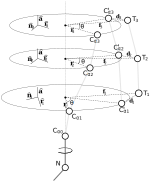
\includegraphics[width=0.75\columnwidth]{figures/ccd_angles}
	\label{fig:ccd_angles}
  \caption{}
\end{figure}

